\documentclass[12pt, twoside]{article}
\documentclass[12pt, twoside]{article}
\usepackage[letterpaper, margin=1in, headsep=0.2in]{geometry}
\setlength{\headheight}{0.6in}
%\usepackage[english]{babel}
\usepackage[utf8]{inputenc}
\usepackage{microtype}
\usepackage{amsmath}
\usepackage{amssymb}
%\usepackage{amsfonts}
\usepackage{siunitx} %units in math. eg 20\milli\meter
\usepackage{yhmath} % for arcs, overparenth command
\usepackage{tikz} %graphics
\usetikzlibrary{quotes, angles}
\usepackage{graphicx} %consider setting \graphicspath{{images/}}
\usepackage{parskip} %no paragraph indent
\usepackage{enumitem}
\usepackage{multicol}
\usepackage{venndiagram}

\usepackage{fancyhdr}
\pagestyle{fancy}
\fancyhf{}
\renewcommand{\headrulewidth}{0pt} % disable the underline of the header
\raggedbottom
\hfuzz=2mm %suppresses overfull box warnings

\usepackage{hyperref}
\usepackage{float}

\title{Algebra 2}
\author{Chris Huson}
\date{October 2023}

\fancyhead[LE]{\thepage}
\fancyhead[RO]{\thepage \\ Name: \hspace{4cm} \,\\}
\fancyhead[LO]{BECA / Huson / Algebra 2: Polynomials \\* 14 November 2023}

\begin{document}

\subsubsection*{2.11 Do Now Quiz: Graphing polynomials}
\begin{enumerate}
    \item Sketch the graphs
        $$g\left(x\right)=x^{3}-14x+2$$
        $$h\left(x\right)=x^{3}+11x^{2}+32x+28$$
    \item What are the zeros of $$f(x)=(x-2)^2 (x+7)(x-8)$$
    \item What is the degree of $f(x)$?
    \item What is the end behavior of $g(x)$?
    \item What are the factors of $h(x)$?
    Which factor has a multiplicity of 2?

    \begin{center}
        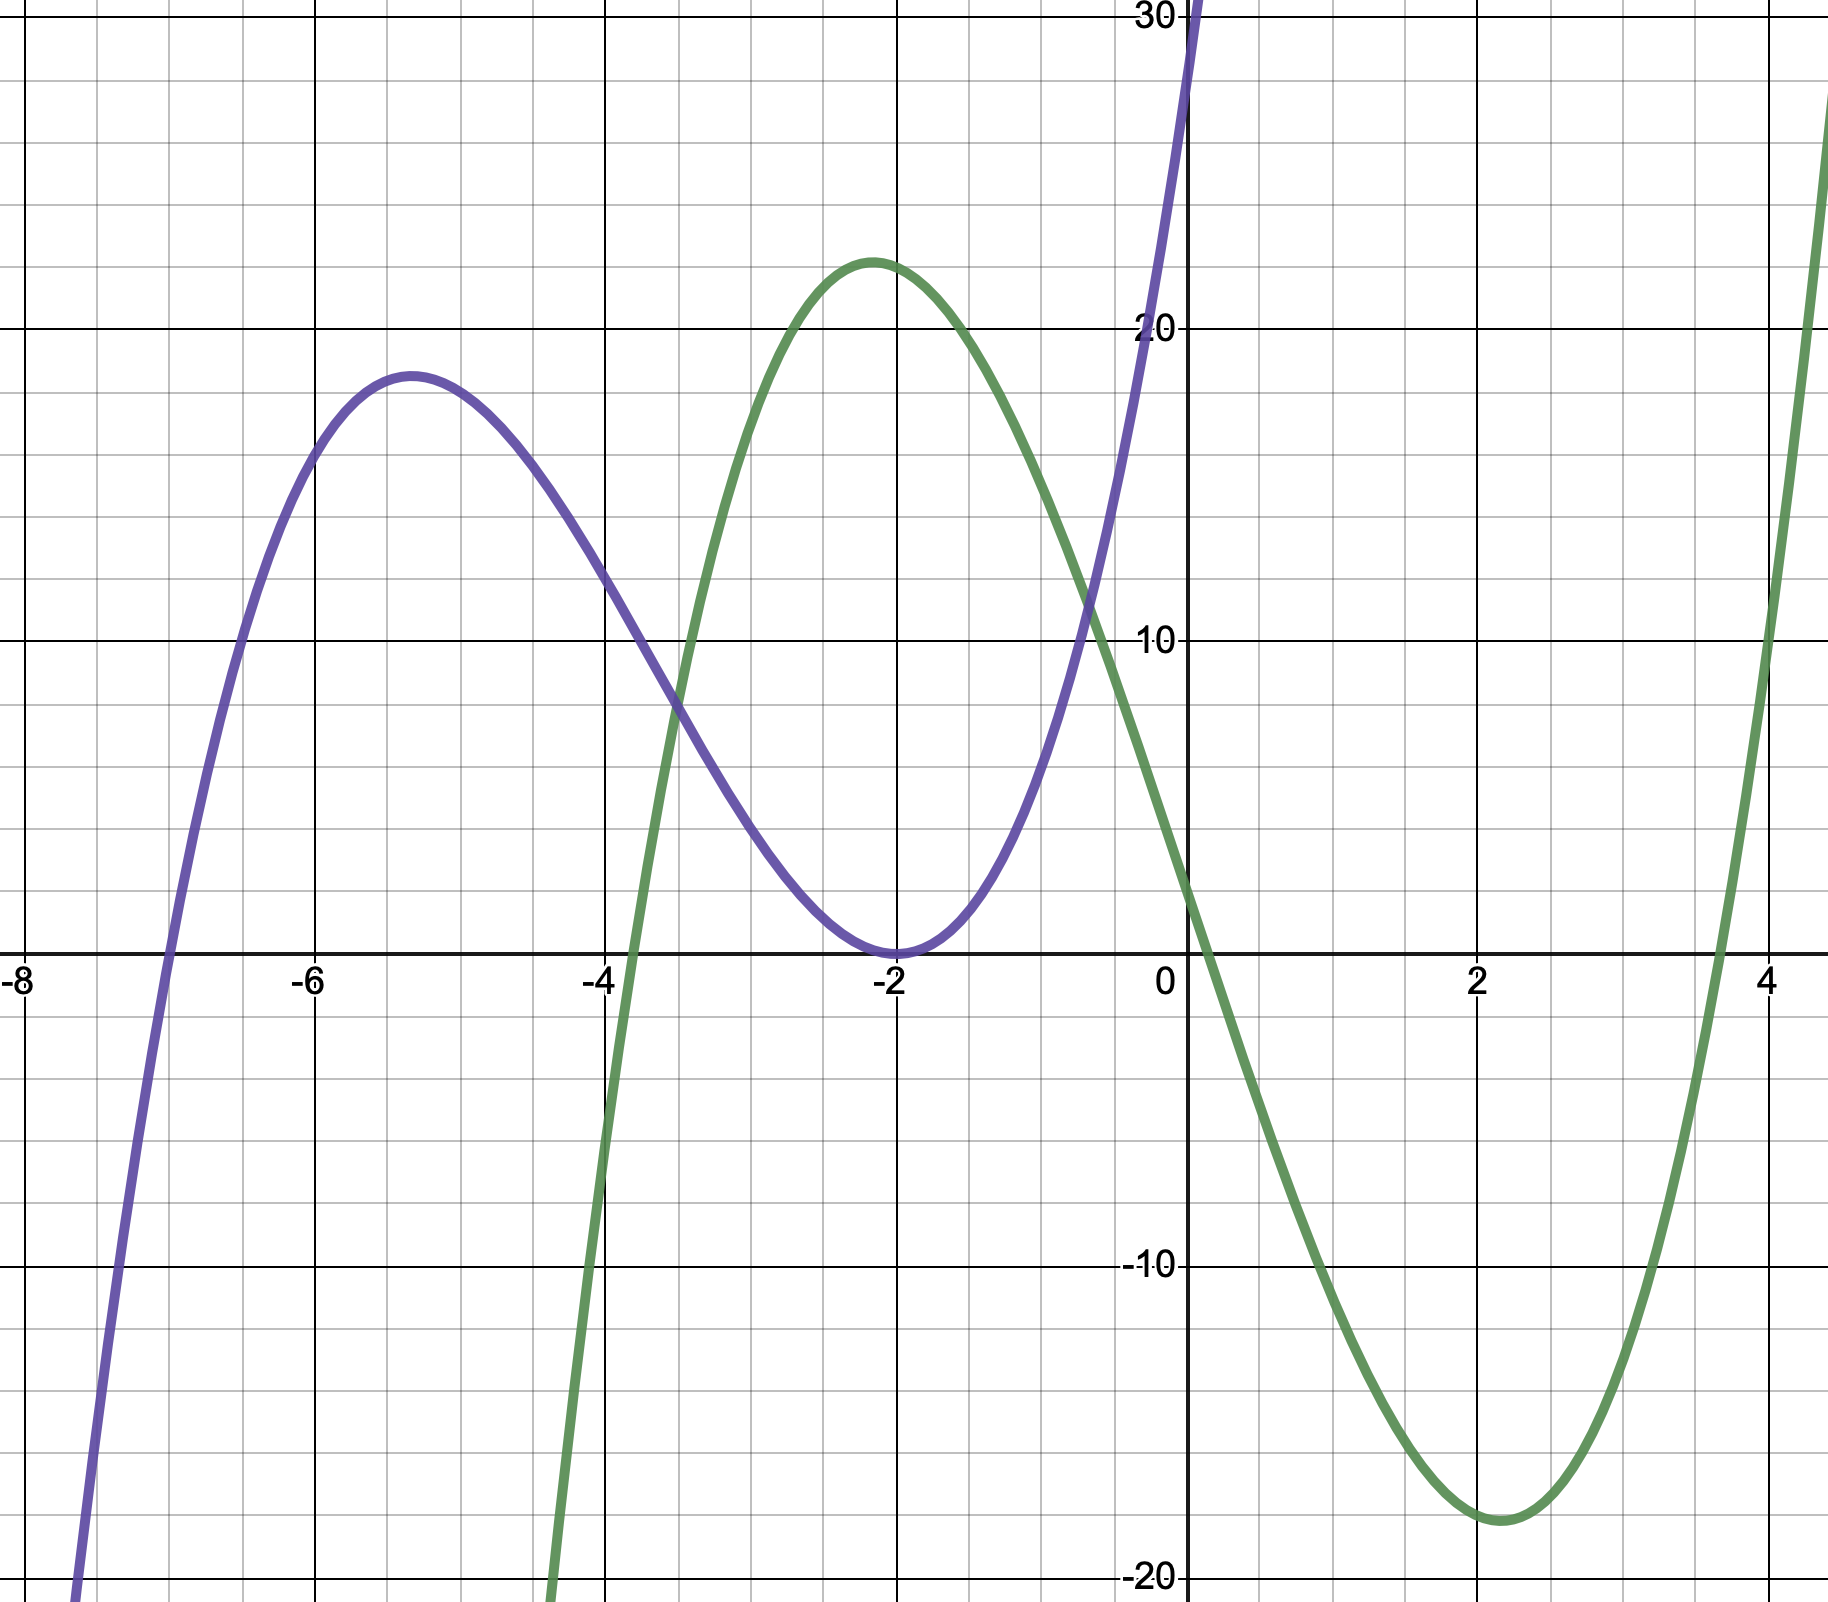
\includegraphics[width=0.6\textwidth]{../graphics/2-11DNQ-graphs.png}
    \end{center}


\newpage
    \item Evaluate each polynomial for the given value of $x$.
    \begin{multicols}{2}
        \begin{enumerate}[itemsep=1cm]
            \item $f(x)=-x^3+12x^2-x+4$, $x=0$ \\[0.25cm] 
            $f(0) = $ \vspace{2cm}
            \item $g(x)=2x^3+11x^2-3x+15$ \\[0.25cm] 
            $g(-8) = $ \vspace{2cm}
        \end{enumerate}
        \end{multicols}
    
    \item The polynomial function $A$, shown below, is used to model the value of an investment account. Three deposits were made which earned interest annually.  $$A(x)=200x^5+300x^4+150x^3$$ 
    \begin{enumerate}[itemsep=1cm]
        \item How much was the first deposit, and how long ago was it made? \vspace{1cm}
        \item If the polynomial is evaluated for $x = 1.04$, what interest rate would that represent \emph{as a percentage}?
        \item Find the value of $A(1.04)$ to the \emph{nearest cent}. \vspace{2cm}
    \end{enumerate}

\subsubsection*{A2-F.BF.2 Write arithmetic and geometric sequences with recursive formulas}
\item Write a recursive formula for each sequence. Use subscript notation.
    \begin{multicols}{2}
    \begin{enumerate}
        \item $3, -6, 12, -24, 48, \dots$
        \item $\displaystyle \frac{3}{4}, \frac{5}{4}, \frac{7}{4}, \frac{9}{4},  \dots$ 
    \end{enumerate}
    \end{multicols}

\newpage
\subsubsection*{A1-A.APR.1 Add, subtract, and multiply polynomials}

\item Find the sum in standard form $(x^3-4x^2+2x+16)+(5x^3-2x^2-3x-12)$ \vspace{2cm}

\item Find the difference $f(x)-g(x)$ as a polynomial in standard form, given \\[0.25cm]
    $f(x)=x^4+2x^3-x-9$ and $g(x)=2x^3+x^2-3x-11$. \vspace{4cm}

\item Multiply the two polynomials $f(x)=3x-2$ and $g(x)=x^2-5x+4$. First complete the grid and then collect terms to find the product as a polynomial in standard form. \\[0.25cm]
\begin{tabular}{|p{1cm}|p{3cm}|p{3cm}|p{3cm}|}
    \hline
     & $x^2$ & $-5x$ & $4$ \\
    \hline
    $3x$ &  & & \\[0.5cm]
    \hline
    $-2$ &  & & \\[0.5cm]
    \hline
\end{tabular} \vspace{4cm}

\item Select all of the expressions that are equivalent to $x^2-5x+6$.
    \begin{multicols}{2}
    \begin{enumerate}
        \item $(x-2)(x+3)$
        \item $(x-3)(x-2)$ 
        \item $(x-5)(x+6)$ 
        \item $(x+2)(x-3)$ 
        \item $(x-6)(x+5)$
        \item $(x+3)(x+2)$ 
        \item $(x-2)(x-3)$
        \item $x^2+5x+6$
    \end{enumerate} 
    \end{multicols}
    \vspace{0.25cm}

\newpage
\subsubsection*{A1-A.APR.3 Identify zeros of polynomials when factorizations are available.}
\item Select all solutions to the equation $(x-3)(2x+1)=0$.
    \begin{multicols}{2}
    \begin{enumerate}
        \item $x=-\frac{1}{2}$
        \item $x=3$
        \item $x=-2$
        \item $x=-0.5$
        \item $x=-3$
        \item $x=\frac{1}{2}$
    \end{enumerate}
    \end{multicols}
    \vspace{0.25cm}

\item Here is the graph of a quadratic function. Which of the following could be its equation?
    \begin{center}
    \begin{tikzpicture}[xscale=0.7, yscale=0.3]
        \draw [thick, ->] (-5.2,0) -- (5.4,0) node [above] {$x$};
        \draw [thick, ->] (0,-14.2)--(0,9.5) node [right] {$y$};
        \foreach \x in {-4,-3,...,4} \draw (\x cm,10pt) -- (\x cm,-10pt) node[below] {$\x$};
        %\foreach \y in {-8,-4,4, 8} \draw (2pt,\y cm) -- (-2pt,\y cm) node[left] {$\y$};
        %\fill (-1,0) circle[radius=0.1] node[above left]{$j$};
        %\fill (3,0) circle[radius=0.1] node[above right]{$k$};
        \draw [thick, <->,smooth,samples=20,domain=-5:4] plot(\x,\x*\x+\x-12);
    \end{tikzpicture}
    \end{center}
    \begin{multicols}{2}
    \begin{enumerate}
        \item $y=(x+3)(x-4)$
        \item $y=(x-3)(x+4)$
        \item $y=(x+3)(x+4)$
        \item $y=(x-3)(x-4)$
    \end{enumerate}
    \end{multicols}

\item Find all of the values of $x$ that make the equation true, the solutions. \\[0.25cm]
$x(x+5)(2x-9)(x-13)=0$. 

\newpage
\item Given the polynomial function $f(x)=2x^4+5x^3-x^2+3x-6$. 
    \begin{enumerate}[itemsep=0.7cm]
        \item What is the degree of the polynomial?
        \item Write down the leading coefficient of $f$.
        \item What is the value of the constant term?
        \item Find $f(1)$.
    \end{enumerate} \vspace{0.7cm}

\item The graph of a polynomial function is shown below. 
    \begin{enumerate}[itemsep=0.7cm]
        \item Write down the $x$-intercepts, the solutions to $f(x)=0$.
        \item Write down the $y$-intercept as an ordered pair.
        \item What term do we use to describe the point $p$ on the plot?
    \end{enumerate} \vspace{0.7cm}
    \begin{center}
    \begin{tikzpicture}[xscale=1, yscale=0.9]
        \draw [thick, ->] (-3.2,0) -- (5,0) node [above] {$x$};
        \draw [thick, ->] (0,-5.2)--(0,6) node [right] {$y$};
        \foreach \x in {-3,...,4} \draw (\x cm,3pt) -- (\x cm,-3pt) node[below] {$\x$};
        \foreach \y in {-4,-2,2,4} \draw (3pt,\y cm) -- (-3pt,\y cm) node[left] {$\y$};
        \fill (-2,0) circle[radius=0.08];
        \fill (1,0) circle[radius=0.08];
        \fill (4,0) circle[radius=0.08];
        \fill (-0.732,5.2) circle[radius=0.08] node[above left]{$p$};
        \draw [thick, <->,smooth,samples=20,domain=-2.3:4.2] plot(\x,{0.5*(\x+2)*(\x-1)*(\x-4)});
    \end{tikzpicture}
    \end{center}

\end{enumerate}
\end{document}